\subsection{Testkonzept Software}\label{sec:testkonzeptSoftware}

Erklärt, welcher Teil wie getestet wird und führt die Ergebnisse mit Auswertung auf.




\subsubsection{PWM Signal}\label{sec: Validierung PWM Signal}
Das PWM Signal wurde mit dem Gleichen Signal wie das LC-Filter validiert. Dabei wurden sowohl die beiden PWM Kanäle mit dem KO aufgezeichnet wie in \autoref{fig Signal PWM Ausgänge} zu sehen ist, sowie das gefilterte Signal. 

\begin{figure}[ht!]
\center
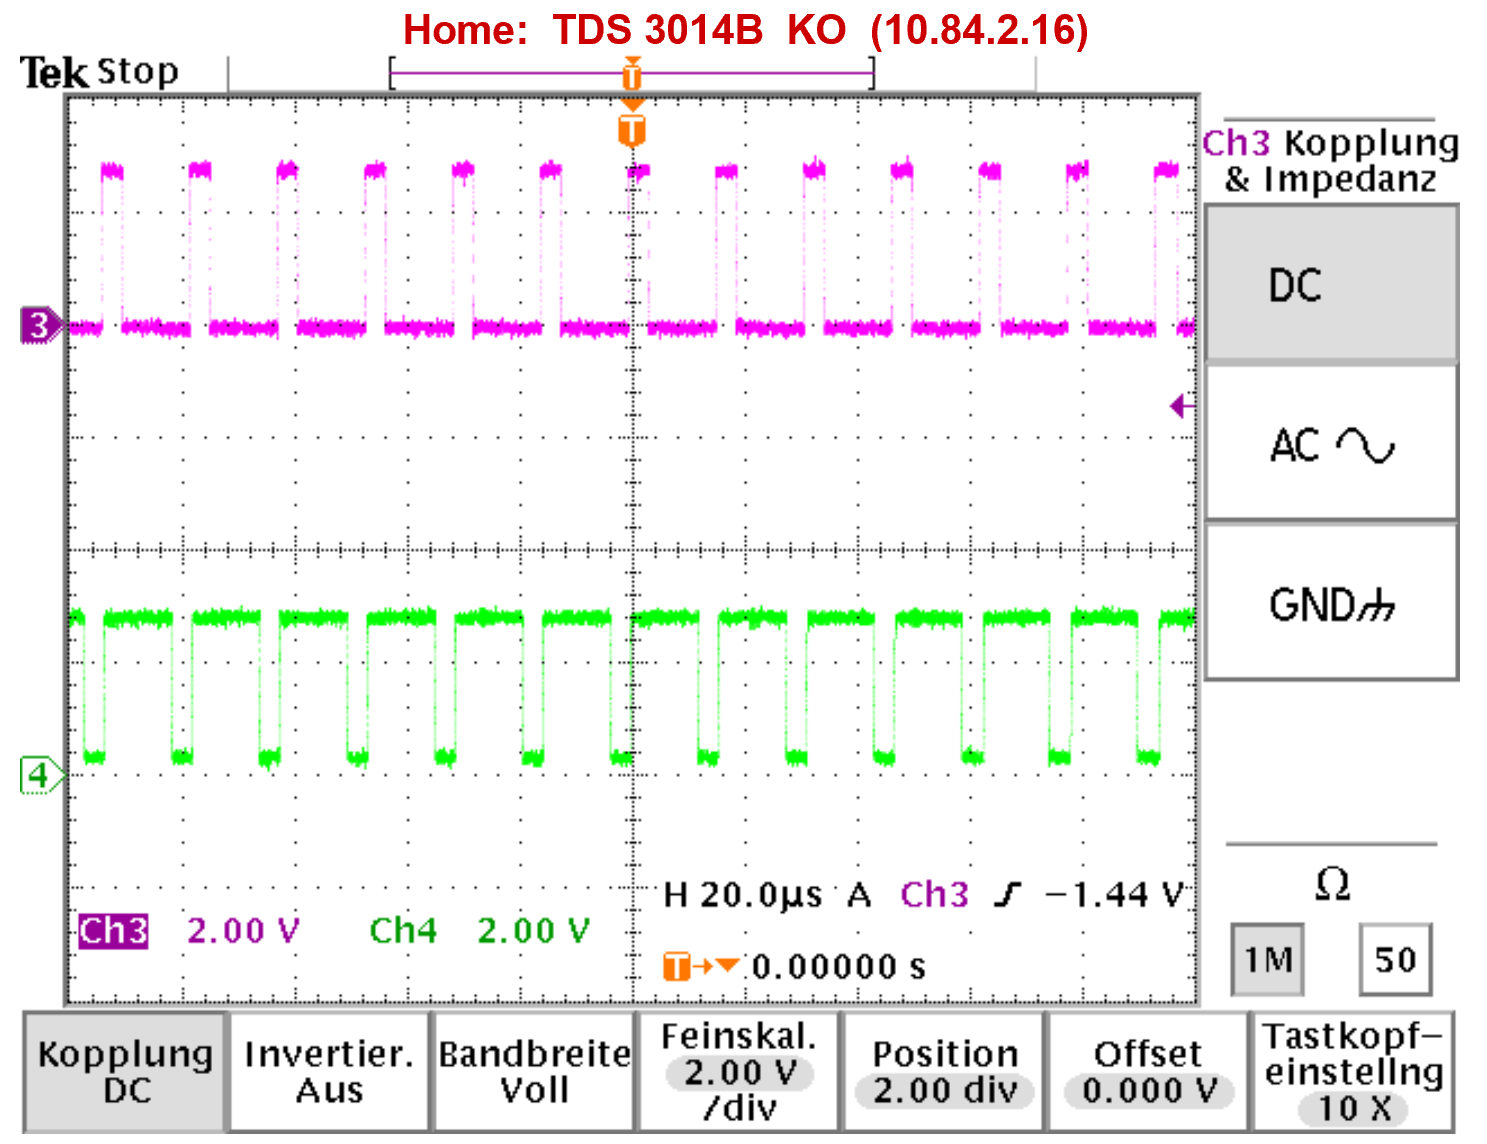
\includegraphics[scale=1.0]{data/PWM_Signal_500Hz_Mono_mit_Infos.png}
\caption{PWM Signal beider PWM Ausgänge}
\label{fig:Signal PWM Ausgänge}
\end{figure}

Aus \autoref{fig:Signal PWM Ausgänge} ist ersichtlich, das die beidem PWM Signale zwar invertiert zu einander sind aber auch Zeitverschoben. Die Zeitverschiebung beträgt knapp $4\mu s$. Dies ergibt keinen hörbaren Effekt und ist somit zu vernachlässigen.

Um die Einstellungen des PWM-Moduls aus \ref{sec:audioPWM} zu validieren wurde wieder ein $500Hz$ Sinus Signal mit dem KO abgebildet.


\begin{figure}
\center
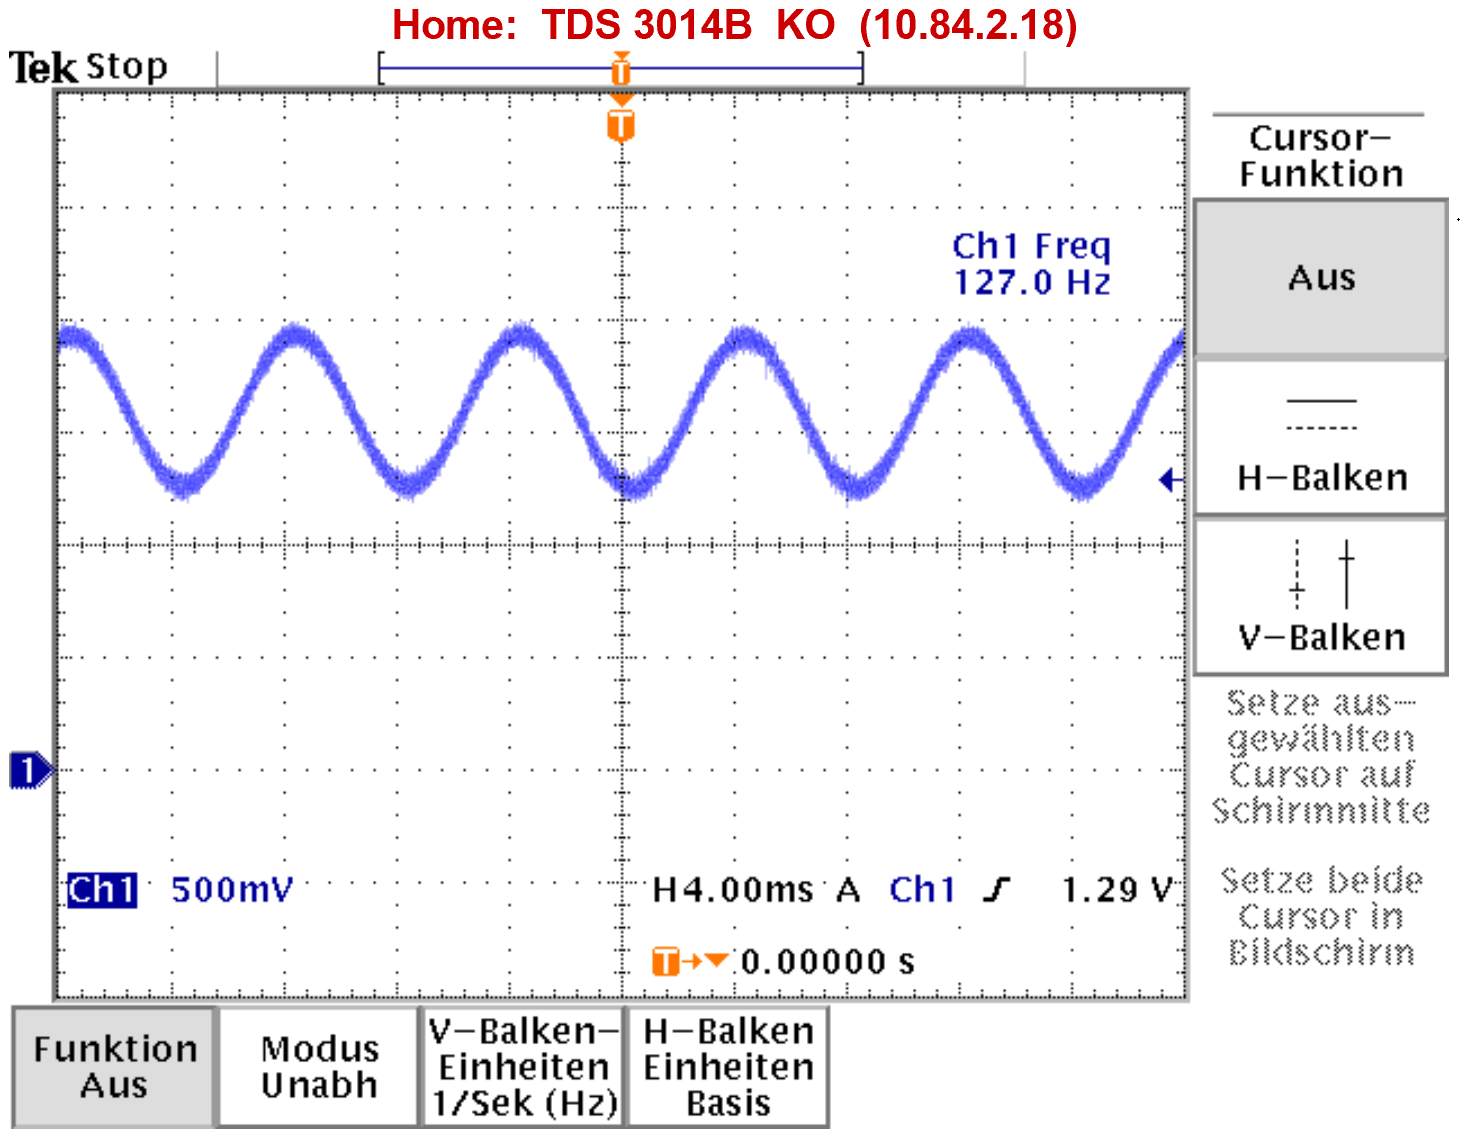
\includegraphics[scale=1.0]{data/TOPVAL_Stereo_500.png}
\caption{PWM auf $32kHz$ eingestellt}
\label{fig:PWM Topval 500 Stereo}
\end{figure}

In \autoref{fig:PWM Topval 500 Stereo} ist ersichtlich, dass die Frequenz des Signals nun nur $127Hz$ anstatt $500Hz$ beträgt. Dies entspricht einem Faktor von ungefähr $4$. Um die $500Hz$ zu erreichen wurde nun der top value aus Kapitel \ref{sec:PWM initialisieren} von $500$ auf $125$ gesetzt. Dies entspricht dem Faktor $4$. In \autoref{fig:PWM Topval 125 Stereo} ist ersichtlich, dass nun das Sinus Signal mit $500Hz$ schwingt.
\newpage

\begin{figure}[ht!]
\center
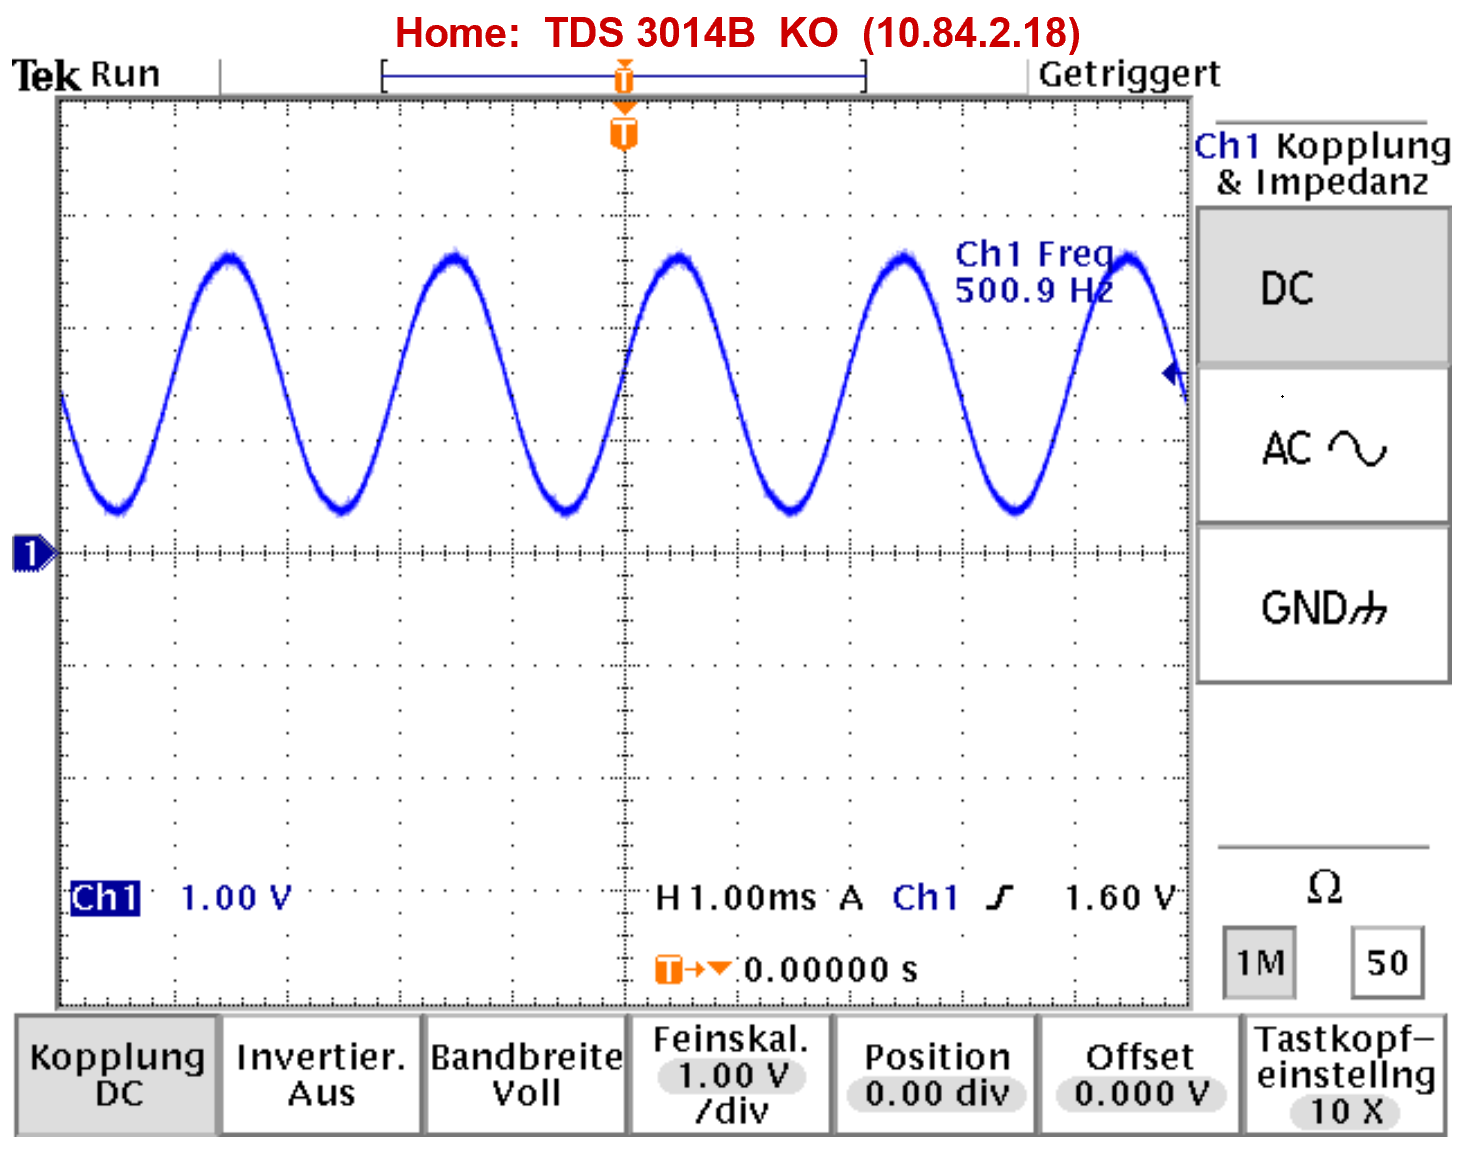
\includegraphics[scale=1.0]{data/TOPVAL_Stereo_125.png}
\caption{PWM auf $128kHz$ eingestellt}
\label{fig:PWM Topval 125 Stereo}
\end{figure}

Da die Berechnungen einen top value von $500$ ergeben, deutet dies auf einen Fehler im Code, in der Audiodatei oder einen Überlegungsfehler hin. Fälschlicherweise wurden diese Tests mit einer stereo Audiodatei durchgeführt. Da nur ein Kanal angesteuert wird, ergibt sich ein Faktor $2$ unterschied zu den Berechnungen. Dieser Test wurde folglich nocheimal mit einer mono Audiodatei durchgeführt. Dabei ergab sich das der top value, wie erwartet, noch um Faktor $2$ vom berechneten Wert abweicht. 


